\documentclass[12pt]{article}

% set margins and spacing
\addtolength{\textwidth}{1.3in}
\addtolength{\oddsidemargin}{-.65in} %left margin
\addtolength{\evensidemargin}{-.65in}
\setlength{\textheight}{9in}
\setlength{\topmargin}{-.5in}
\setlength{\headheight}{0.0in}
\setlength{\footskip}{.375in}
\renewcommand{\baselinestretch}{1.0}
\linespread{1.3}

% load miscellaneous packages
\usepackage{csquotes}
\usepackage[american]{babel}
\usepackage[usenames,dvipsnames]{color}
\usepackage{graphicx,amsbsy,amssymb, amsmath, amsthm, MnSymbol,bbding,times, verbatim,bm,pifont,pdfsync,setspace,natbib}

% enable hyperlinks and table of contents
\usepackage[pdftex,
bookmarks=true,
bookmarksnumbered=false,
pdfview=fitH,
bookmarksopen=true,hyperfootnotes=false]{hyperref}

% define environments
\newtheorem{definition}{Definition}
\newtheorem{fact}{Fact}
\newtheorem{result}{Result}
\newtheorem{proposition}{Proposition}



\begin{document}
\title{Accident's Team: The Effect of Establishment Size on Injury Rate}
\author{Anna\thanks{Syracuse University, Economics Department. Email: kbuzard@syr.edu.} \and Tomoyoshi\thanks{abc} \and Yuhan\thanks{abc}\and Will}
\date{\vskip-.1in \today }
\maketitle

\vskip.3in
\begin{center} {\bf Abstract} \end{center}

\begin{quote}
This research investigates the impact of establishment size on workplace safety, specifically examining the correlation between establishment size and the rate of injuries. Motivated by the role of workplace safety in employee well-being and business success, our study employs data from the Occupational Safety and Health Administration (OSHA) to explore this relationship. The theoretical foundation suggests that larger establishments may experience fewer injuries per worker due to potential economies of scale in OSHA inspections and safety practice implementation costs. Preliminary findings challenge the common hypothesis and indicate a weak or non-existent correlation. Through a thorough literature review, theoretical analysis, and empirical examination, this paper contributes valuable insights to the discourse on workplace safety dynamics.
\end{quote}

\bigskip
\section{Introduction} \label{sec:introduction}

Workplace safety is a critical concern that profoundly impacts both individuals and organizations. As the modern workforce continues to evolve, understanding the dynamics of workplace safety becomes increasingly important. In this context, our research investigates the nuanced relationship between establishment size and workplace injuries. The motivation for this study arises from the paramount importance of maintaining safe working conditions, not only for the well-being of employees but also for the overall success and reputation of businesses.

Ensuring workplace safety is not only a moral imperative but also a strategic move for organizations aiming to attract and retain talent. The ability to create and maintain a safe work environment is central to fostering a healthy and productive workforce. In this paper, we address the question of whether there exists a correlation between establishment size and the rate of workplace injuries. By leveraging data collected by the Occupational Safety and Health Administration (OSHA), we seek to contribute valuable insights that transcend specific industries and job types.

The choice of this research topic is driven by the need for an understanding of the factors influencing workplace safety. While numerous studies focus on this subject, our research stands out by examining diverse and complex data. Our primary objective is to answer whether establishment size plays a significant role in determining the rate of workplace injuries. To achieve this, we conduct a thorough analysis of variables such as total injuries and injury types across different decile groups based on establishment size.

Preliminary findings challenge the common hypothesis that larger establishments would experience fewer injuries per worker. Instead, our results suggest a weak or non-existent correlation, prompting further exploration into the nuances of this relationship. Overall, our findings are important in understanding the layout of work place safety and offers insight for new ideas. 

\section{Literature Review} \label{sec:literature}

Our paper takes a close look at what makes workplaces safe and what can cause more accidents. We started by looking at some old studies, like the ones by (Viscusi, 1979)and (Smith, 1979), which asked if having safety inspections at work actually made things safer. They found that right after inspections in 1973, workplace injuries went down by 17%, but the next year in 1974, things didn't really look any different. 
This makes it kind of Difficult to say for sure if inspections help prevent accidents or not. (Li Li, 2019) touches on the most recent data and suggests that OSHA has a positive impact on worker safety.  

Then, there's a study by (Li L., 2019) that checked if being in a labor union means fewer accidents happen at work. It seems logical because unions are supposed to look out for workers' safety. But, surprisingly, the study showed that just being in a union didn't really change the number of accidents. The type of job people do also matters. (Charles K.K Johnson M.S., 2019)showed that in mining, when there's a sudden increase in demand for what they're digging up, there tend to be more accidents. This is probably because when companies are really busy, they might not focus as much on following safety regulations. 

(DAVID I. LEVINE, 2012)suggested that companies that make their workplaces safer could end up doing better in the long run since more people would want to work in a place that's known for being safe. 
What makes our paper stand out is that we didn't just look at one place or one kind of job—we looked at lots of different data from all over. This way, we can really understand what's going on with safety at work everywhere. 

\section{Theoretical Analysis}
\label{sec:theory}

In this paper, we examine the hypothesis that larger establishments are likely to experience fewer injuries per worker compared to smaller establishments. This assertion is grounded in the concept of economies of scale, particularly in terms of Occupational Safety and Health Administration (OSHA) inspections and the costs associated with implementing or improving safety practices. Larger establishments, benefiting from economies of scale, may find it more cost-effective to invest in comprehensive safety measures and OSHA compliance. This financial advantage could potentially lead to enhanced safety practices and a reduced likelihood of workplace injuries. In contrast, smaller establishments, facing comparatively higher costs per unit, might be incentivized to adopt practices that prioritize worker safety to a lesser extent. This theoretical framework provides a foundation for our empirical analysis of the relationship between establishment size and workplace injuries.
\section{Data}
\label{sec:data}

The data being used for this research project is from the Occupational Safety and Health Administration (OSHA). OSHA collects data across different establishments each year in hopes to measure workplace safety. This data is cross sectional data that has more than 20 variables across approximately 350,000 establishments. Our data was sourced from Professor Singleton’s work on workplace safety and violations.
   
We are testing the relationship between establishment size and number of injuries. For this research project, we are using several of the given variables and also generating our own variables to help create a more robust analysis. To begin, our first goal is to make sure the data is clean and that it will generate usable conclusions. Using Stata, we worked on making sure the data resolved logically, meaning that we would remove data based on an equation that identified ratios of variables that were impossible to achieve, likely put in place because of a procedural issue with reporting. For the variable annual\_average\_employees, we determined that values below zero, above or equal to the total\_hours\_worked value in the same entry, or valued at 123456 were to be replaced with a null value. We also determined that for the variable total\_djtr\_days, if the value was above or equal to total\_hours\_worked in the same entry, or if it was below zero, they were to be replaced with a null value. This made little to no difference in the final analysis.
    
After completing the data fix, we generated variables that made sense for our hypothesis. For example, we know we want to focus on the Total\_Injuries variable but in bigger establishments there is bound to be more total injuries due to the increased number of employees. To combat this issue, we generate a new variable entitled inj\_rate this variable creates a per establishment rate based on the number of employees at that establishment. To do this we calculated the quotient of total\_injuries over the annual\_average\_employees. In doing so, we now can look at the injury rate across all establishment sizes and compare that raw data. We replicated this process across all the different injury types: skin disorders, respiratory issues, and poisonings. Professor Singleton used a similar method in his paper “The Effect of Workplace Inspections on Worker Safety”, and due to the origin of our data and guidance, we proceeded with a similar route.

The final change we made to the data was creating the variable decile This variable uses annual\_average\_employees and separates it into ten groups based on percentile. This variable is the most efficient way to answer our hypothesis because to find the relationship between establishment size and workplace injuries we need to come to an understanding of what “establishment size” means. For our research, establishment size is based on the number of employees and is separated into 10 groups. This promotes a more holistic understanding of establishment size and the trends associated with it.

\section{Results}
\label{sec:result}

In this section, we dive into the analysis of our data-set, aiming to understand the relationship between establishment size and workplace injuries. To begin our analysis, we created a bar chart (Figure 1) comparing the Inj\_Rate means across each of our decile groups to see if injury rate changed based on establishment size. Our decile groups, as discussed in the data section are grouped by percentile and range from nine to over a million. It is important to note that from decile one to decile nine the range is 244, this gives context to the real sizes of these establishments. From first glance there was not a clear trend within the data. We then proceeded to run a simple correlation test between the two variables, to present a numerical understanding of what we were already viewing in our bar chart. We found a correlation coefficient of -0.0136 which suggests an extremely weak negative correlation. While the negative sign indicates a negative relationship, the small magnitude implies that the relationship is not practically significant. In other words, the variables have little linear association. To better understand this variable, we also used a summary command. We found a mean Injury Rate of .0352, Median of .017, and a Standard Deviation of .0882. Based on this information a substantial number of the observations is between 0 and 0.3. One piece of the summary statistics that stood out to us was the outliers, 7.5, 9.37, 10.76, and 28. These data points are substantially outside of our inter-quartile range. These data points also imply that a hypothetically establishment with 1 worker is getting injured 7 to 28 times. These summary statistics offer insight into the accuracy of our data and can also lead us to questions about the data collection process.
\begin{figure}
    \centering
    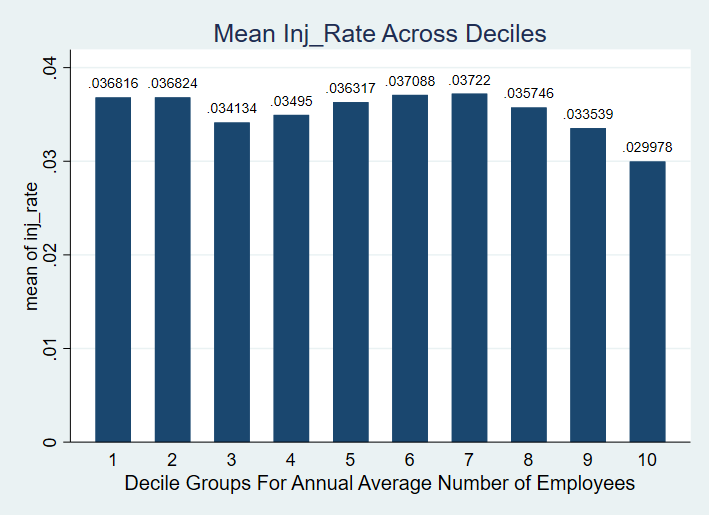
\includegraphics[width=0.7\linewidth]{Inj_RateDecileBar (3).png}
    \caption{Mean Injury Rate Across Decile Groups}
    \label{Figure 1:}
\end{figure}

For the second part of our analysis, we aimed to understand more about the data passed total injuries recorded. The reasoning for this is because the variable total\_injuries encapsulates several different injury types, all with different relationships with the decile variable. To provide more insight on this notion we have included three new variables, Total\_Poisonings\_Rate,  Total\_Skin\_Disordersrate, and Total\_Respiratory\_Conditionsrate. To begin this section of analysis, we created Figure 2: The Distribution of The Total Poisoning Rate across Decile Groups. From a first glance the initial eye sore is the first decile group and its domination over the other nine. To explore this outlier, we first looked at summary statistics and found that the mean poisoning rate was .0000231 and the standard deviation was .0021069, and the median was 0. We then used tabulate and codebook to look through the data for possible outliers causing the smallest decile group to have the highest rate. We found that one observation had a Skin Disorder rate of exactly 1, implying that every person at that establishment had a skin disorder. Finally, we ran a correlation test and found a correlation coefficient of -.0025 which does not support our hypothesis because it highlights a subtle negative correlation between the two variables, however the correlation coefficient is not substantial enough to show obvious causation.  

\begin{figure}
    \centering
    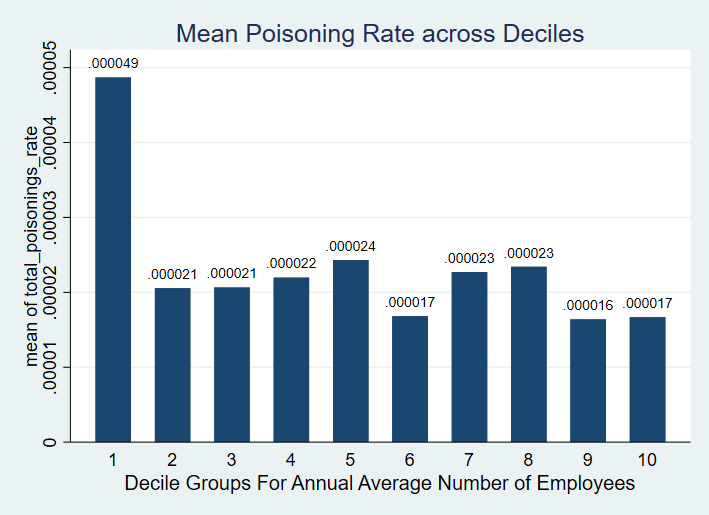
\includegraphics[width=0.7\linewidth]{PoisoningsDecileBar (2).png}
    \caption{The Distribution of The Total Poisoning Rate across Decile Groups}
    \label{Figure 2:}
\end{figure}


The next variable we looked at was the total\_skin\_disordersrate. As shown in Figure 3, we created a bar chart to analyze the relationship between the skin disorders rate and establishment size. At first glance it is hard to see if there is a correlation between the two variables, so we ran a correlation test and found a correlation coefficient of .0031. A correlation coefficient of 0.0031 suggests a very weak positive correlation between the two variables and it's important to note that correlation does not imply causation. This correlation coefficient supports our hypothesis but there may be other factors that might influence the relationship between the variables. Additionally, the strength and direction of the relationship can vary based on the context of the data. To look further into this relationship we ran a summary command to see if there was anything worth noting, we found a mean skin disorder rate of .0001993, a range of 0 to 1, the standard deviation is .04745, and a median of 0. Compared to the main injury rate and the other types of injuries within our data this variable has a much smaller distribution with no huge outliers. The median of 0 also implies this injury does not occur much across establishments. 

\begin{figure}
    \centering
    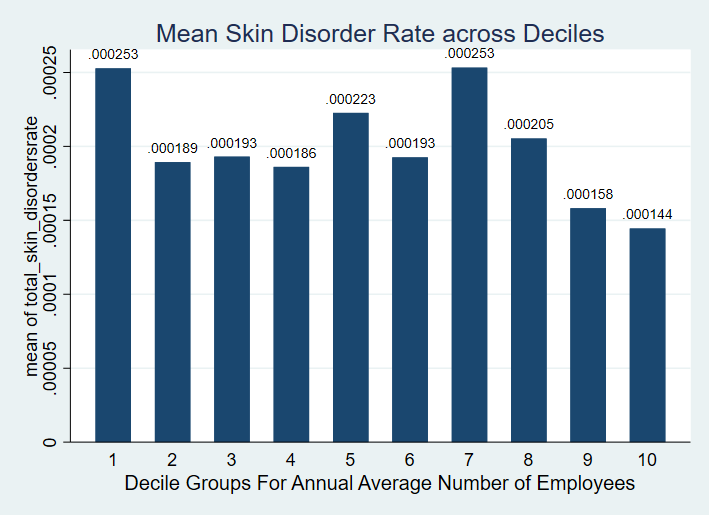
\includegraphics[width=0.7\linewidth]{SkinDecileBar (1).png}
    \caption{Mean Skin Disorder Rate across Decile Groups}
    \label{Figure 3:}
\end{figure}

The last variable we looked at was total\_respiratory\_conditionsrate, this variable measures the rate of respiratory issues reported within a year over the number of employees at a given firm. We created a bar chart to highlight the relationship between this variable across our decile groups and saw a clear negative correlation between respiratory conditions and decile groups, which is highlighted in Figure 4. To confirm this, we ran a correlation test and found a correlation coefficient of .0286. In our case, the value is close to 0, indicating a weak positive correlation. This suggests that as one variable increases, the other tends to increase slightly, but the relationship is not strong. The decile group with the highest respiratory rate was decile 8 which leads to questions about why? Is the correlation of this injury type sector based? To finalize our analysis, we ran a summary command and found a slightly large distribution with a range from 0 to 4.625.Implying that this variable may have more outliers than skin disorder injuries. We also found a mean of .00633, a standard deviation is .04745, and the median is 0. This shows that many of the establishments avoided respiratory issues but certain establishments must have been more prone than others with the range spanning so wide. 


\begin{figure}
    \centering
    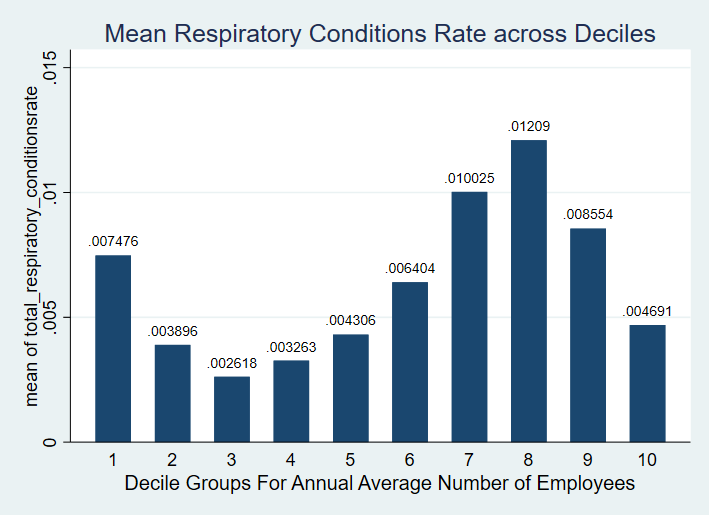
\includegraphics[width=0.7\linewidth]{RespiratoryDecileBar (1).png}
    \caption{Mean Respiratory Rate across Decile Groups}
    \label{Figure 4:}
\end{figure}

Finally, we wanted to include more about the variance of our data and provide further insight on the issues this data had with outliers. In doing so we created box plot to examine the different decile's injury rates to see if there were any trends in variance that were worth noting. The main takeaway from  this graph was that some decile groups had more outliers than others. For example, decile 1 had one observation in with an injury rate of 28. Decile 1 is the establishments with eight to nineteen people, meaning that some of these firms were having all eight employees injured 28 times. We also noticed that there was no trend in variance based on decile. This was not shocking based on the amount of outliers across the board but did highlight issues with data collection across all establishment sizes. This was also explored through the inclusion of median and mean comparison in our summary statistics because it highlights skewed distribution in the data and the large variance across all deciles. 

\begin{figure}
    \centering
    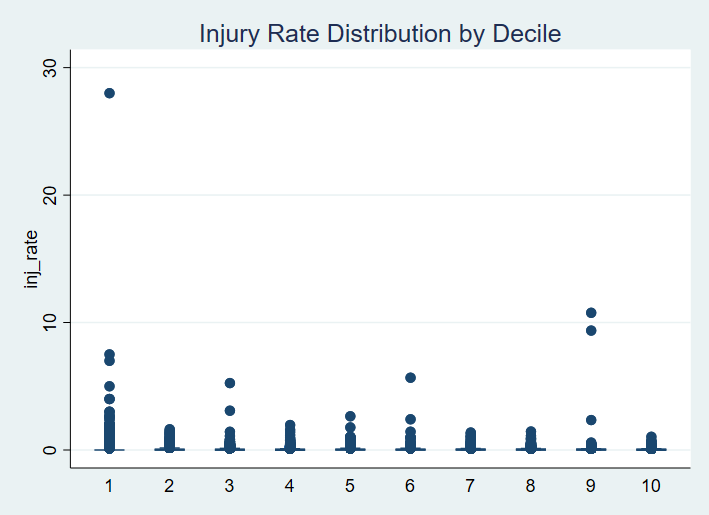
\includegraphics[width=0.8\linewidth]{InjRateBox.png}
    \caption{Injury Rate Distribution By Decile}
    \label{fig:enter-label}
\end{figure}

The main takeaway from this analysis is that this data has extreme outliers and minimal correlation between injury rates and establishment size. Our hypothesis is not supported enough by this data set, however, this information is extremely helpful in pointing out potential hypotheses for future work on workplace safety and offers insight on injuries that are unique to certain lines of work.  



\section{Discussion}
\label{sec:discussion}

    The data analysis and results above display that there are potential issues existed within the data set. The data collected by OSHA are self-reports of number of incidents from individual firms. The different policies that each firm has on reporting and defining an accident may lead to the outliers in variables studied. And there is no obvious way to avoid these extreme cases for data collections. To continue the research, exploring on new data resources which contain the accidents report for different types and size of firm may resolve the abnormal cases. In addition, it is also worth studying about the variable of total\_respiratory\_condition. In the year case of 2023, this variable has an unusual rate of respiration related accidents per capita, which may be due to the aftermath of COVID-19. In future study, a deeper exploration on the total\_respiratory\_condition in the year case of 2019, 2020, 2021, 2022 is necessary to check on the influence of COVID-19. And by studying the injuries rate in these year cases, it helps determine the correlations on the external factors and the injuries rate per capita, firm size.


\section{Conclusion}
\label{sec:conclusion}

In this research, we examine whether there is a correlation between injuries rate and firm size by using data collected from OSHA. We calculated the injuries rate per capita and the rate of other variables such as total skin disorders, total respiratory conditions, and etc, to compare them with the ten deciles of annual average employees. The results demonstrate that there is no, or extremely weak correlation of -0.0136 between injuries rate and firm size. Our hypothesis, which is larger establishments will experience less injuries per worker than smaller establishments, has been proved invalid. The conclusion on hypothesis may be presented with more certainty if additional time is given to test on data from a different year case, or new resources. When considering if firm size impacts workplace accidents rates, other uncontrollable factors such as the report policies, the process of data collections, the external environment, add extra unknown variables to the research and affect the result with outliers. Solving the potential extreme cases within the data would be an essential beginning for researching workplace accidents.

\newpage
\section*{Bibliography}
\singlespacing
\setlength\bibsep{0pt}


\newpage
\section*{Appendix A. Placeholder} \label{sec:appendixa}
\addcontentsline{toc}{section}{Appendix A}

\end{document}